\input{../YKY-preamble.tex}
% \usepackage[no-math]{fontspec}
% \setmainfont[BoldFont=Alibaba_Sans_Regular.otf,ItalicFont=Alibaba_Sans_Light_Italic.otf]{Alibaba_Sans_Light.otf}

\usepackage[backend=biber]{biblatex}
\bibliography{../AGI-book}

\usepackage[active,tightpage]{preview}		% for continuous page(s)
\renewcommand{\PreviewBorder}{0.5cm}
\renewcommand{\thempfootnote}{\arabic{mpfootnote}}

\usepackage[absolute,overlay]{textpos}		% for page number on upper left corner

\usepackage{color}
% \usepackage{mathtools}
\usepackage[hyperfootnotes=false]{hyperref}

% \usepackage[backend=biber,style=numeric]{biblatex}
% \bibliography{../AGI-book}
% \renewcommand*{\bibfont}{\footnotesize}

\usetikzlibrary{shapes}
% \usepackage[export]{adjustbox}	% ??
\usepackage{verbatim} % for comments
% \usepackage{newtxtext,newtxmath}	% Times New Roman font

% \titleformat{\subsection}[hang]{\bfseries\large\color{blue}}{}{0pt}{} 
% \numberwithin{equation}{subsection}

\newcommand{\underdash}[1]{%
	\tikz[baseline=(toUnderline.base)]{
		\node[inner sep=1pt,outer sep=10pt] (toUnderline) {#1};
		\draw[dashed] ([yshift=-0pt]toUnderline.south west) -- ([yshift=-0pt]toUnderline.south east);
	}%
}%

\newcommand\reduline{\bgroup\markoverwith{\textcolor{red}{\rule[-0.5ex]{2pt}{0.4pt}}}\ULon}

%\DeclareSymbolFont{symbolsC}{U}{txsyc}{m}{n}
%\DeclareMathSymbol{\strictif}{\mathrel}{symbolsC}{74}
%\DeclareSymbolFont{AMSb}{U}{msb}{m}{n}
%\DeclareSymbolFontAlphabet{\mathbb}{AMSb}
%\setmathfont{lmroman17-regular.otf}
\DeclareMathOperator*{\argmin}{arg\,min}
\DeclareMathOperator*{\argmax}{arg\,max}

% \usepackage[most]{tcolorbox}
%\tcbset{on line, 
%	boxsep=4pt, left=0pt,right=0pt,top=0pt,bottom=0pt,
%	colframe=red,colback=pink,
%	highlight math style={enhanced}
%}
%\newcommand{\atom}{\vcenter{\hbox{\tcbox{....}}}}

\let\oldtextbf\textbf
\renewcommand{\textbf}[1]{\textcolor{blue}{\oldtextbf{#1}}}

\newcommand{\logic}[1]{{\color{violet}{\textit{#1}}}}
\newcommand{\underconst}{\includegraphics[scale=0.5]{../2020/UnderConst.png}}
\newcommand{\KBsymbol}{\vcenter{\hbox{\includegraphics[scale=1]{../KB-symbol.png}}}}
\newcommand{\token}{\vcenter{\hbox{\includegraphics[scale=1]{token.png}}}}
\newcommand{\proposition}{\vcenter{\hbox{\includegraphics[scale=0.8]{proposition.png}}}}

\begin{document}

\begin{preview}

\title{\vspace{-1.5cm} \bfseries\color{blue}{\LARGE AGI from the perspective of\\
	categorical logic}}

\author{YKY} % Your name
% \date{\vspace{-2cm}} % Date, can be changed to a custom date

\maketitle

\setcounter{section}{-1}
\newcounter{mypage}
\setcounter{mypage}{0}

% (1) Circled page number on upper left corner
\begin{textblock*}{5cm}(2.1cm,2.3cm) % {block width} (coords) 
{\color{red}{\large \textcircled{\small \themypage}}}
\addtocounter{mypage}{1}
\end{textblock*}

\begin{minipage}{\textwidth}
\setlength{\parskip}{0.4\baselineskip}

\section{Basics}

\begin{itemize}
	\item 首先 范畴逻辑 的中心思想是 Curry-Howard isomorphism,不明白这点无从入门。
	\item Curry-Howard 同构 指的是: 用数学上 函数的	模拟 逻辑上的蕴函关系 $A \Rightarrow B$.
	\item 由于这个对应关系,逻辑上的 命题 A 对应与函数的 domain A.
	\item 也就是说,命题对应于某种类似 空间 的东西。
	\item 而那空间里的物体,就是所谓 proof objects,即该命题的证明。
	\item 这样说有点难懂,但其实我们天天都面对这种东西:那就是 神经网络。
	\item 它将某些 向量 映射到 别的向量,向量 就是 proof,
	\item 某个向量周围的空间(在一定误差下)表示 同一概念,
	\item 所以不妨把那邻域的空间看成是一个 逻辑命题。
	\item 这种做法实在太明显也太自然了。
\end{itemize}

做了这个对应之后,逻辑上 $A \Rightarrow B$ 的真值表,很奇妙地跟函数空间的基数 (cardinality) 吻合:
\begin{equation}
\label{truth-table:material-implication}
\begin{tabular}{|c|c|c|c|}
\hline 
$A$ & $B$ & $A \Rightarrow B$ & $B^A$ \\ 
\hline \hline 
0 & 0 & 1 & $0^0 = 1$ \\
\hline 
0 & 1 & 1 & $1^0 = 1$ \\ 
\hline 
1 & 0 & 0 & $0^1 = 0$ \\ 
\hline 
1 & 1 & 1 & $1^1 = 1$ \\ 
\hline 
\end{tabular} 
\end{equation}

这也让我们更有信心,Curry-Howard 同构是将逻辑 数学化 的正确方向。

范畴逻辑 的目的就是:利用范畴论里各种抽象的工具,描述 逻辑的结构。

基于 命题 = 某种空间,那么 很自然地,我们可以用范畴里的 物体 (objects) 代表命题,这种做法更为一般。
用范畴论 里的 products 表达逻辑上的 $\wedge$ 或 $\vee$,exponentiation 表达 逻辑上的 $A \Rightarrow B$,这也同时是范畴里的 morphism $A \rightarrow B$.

$\forall$ 和 $\exists$ 是 某种 variable substitution map 的 adjoint,因为 adjunction 也是数学上常见的结构:
\begin{equation}
\vcenter{\hbox{\includegraphics[scale=0.8]{../2020/Lawvere-cylindrification-forall.png}}}
\quad
\vcenter{\hbox{\includegraphics[scale=0.8]{../2020/Lawvere-cylindrification-exists.png}}}
\end{equation}
(这比较复杂,但我以前也讲解过了,重要的是理解整体的概念,暂时不要迷失在细节里)

\end{minipage}
\end{preview}

\begin{preview}
\begin{textblock*}{5cm}(2.1cm,2.3cm) % {block width} (coords) 
	{\color{red}{\large \textcircled{\small \themypage}}}
	\addtocounter{mypage}{1}
\end{textblock*}

\begin{minipage}{\textwidth}
	\setlength{\parskip}{0.4\baselineskip}

\section{Where is GPT?}

逻辑 谓词 (predicates) 表示为 纤维结构 (fibration), 即以一个 base 空间 对某个上层空间做 ``indexing,'' 可以看下图理解:
\begin{equation}
\vcenter{\hbox{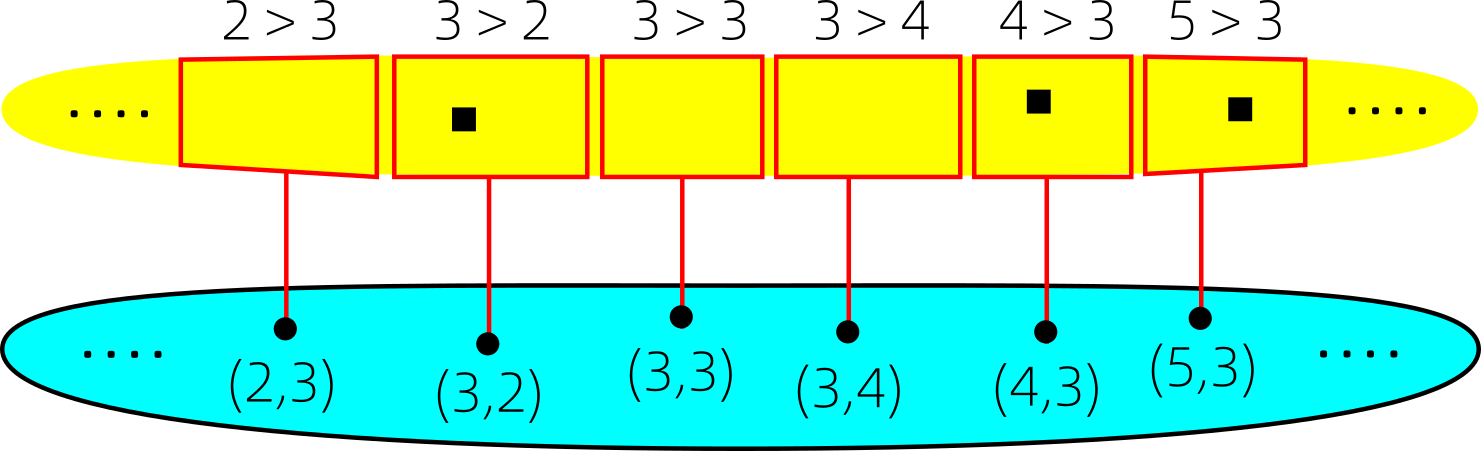
\includegraphics[scale=0.6]{sheaf-of-propositions-over-numbers.png}}}
\end{equation}

我们考虑的是某个二元关系 ``$>$'', 所以底层 base space 是 $\mathbb{N} \times \mathbb{N}$ 即一对对的自然数。 我们可以构成 谓词逻辑命题 $>(a,b)$,而因为 Curry-Howard,这些命题是一些 “空间”,即上层那些黄色的方格。 每个方格是一个命题,它可以有或没有 证明,即黑色的小方格 ■。

上面 所有黄色方格的 并集 就是一个 层 (sheaf),它是所有命题的空间 $\mathbb{L}$. GPT 就是一个将 命题 映射到 命题 的 逻辑推论算子 (logic consequence operator). 但注意: GPT 是一种 set-valued mapping, 它作为函数的 domain 不是 $\mathbb{L}$,而是 命题的 集合 的空间,亦即 power set of L 或者可以记作 PL:
\begin{equation}
\vcenter{\hbox{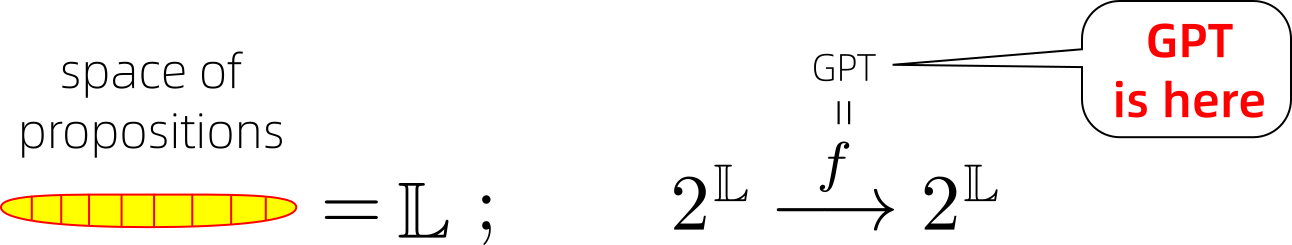
\includegraphics[scale=0.9]{GPT-is-here.png}}}
\end{equation}

大家知道了「GPT 在哪里」,是不是觉得清晰了很多? 至少我是这样觉得的,因为我非常熟悉 logic-based AI, 我习惯了从这个角度 理解我需要用的数学。

\end{minipage}
\end{preview}

\begin{preview}
\begin{textblock*}{5cm}(2.1cm,2.3cm) % {block width} (coords) 
{\color{red}{\large \textcircled{\small \themypage}}}
\addtocounter{mypage}{1}
\end{textblock*}

\begin{minipage}{\textwidth}
\setlength{\parskip}{0.4\baselineskip}

\section{What is HoTT?}

由于 Curry-Howard 说 命题 是 某种「空间」,那么这空间会不会有 拓扑结构? 最近英年早逝的天才 Voevodsky 提出了 命题空间内有 homotopy 的结构,那就是 HoTT (homotopy type theory) 的基本思路。
\begin{equation}
\vcenter{\hbox{\includegraphics[scale=0.4]{../2020/Voevodsky.jpg}}} \nonumber
\end{equation}

以我肤浅的理解,一个命题 要么有证明 或没有证明,如果有证明的话,A 证明和 B 证明 是没有分别的。 但 HoTT 提出 它们可以有区别。 在一个命题的内部空间里,path-connected 的两个点 (proofs) 被视为 identical,但这空间内可以有不是 path-connected 的空间结构,那么 两个 proofs 就可以视为 不相同。

一个例子是: 西方古代将 金星 视为 morning star 和 evening star,而不知道它们其实是同一颗星。 这就是 intension 和 extension 的不同(意指和实际的外延不同),涉及 内涵逻辑 (intensional logic) 的问题,它的 语义可以用 模态逻辑 (modal logic) 和 Montague semantics 处理,详细可参看这篇文章: https://plato.stanford.edu/entries/logic-intensional/ 

\begin{equation}
\vcenter{\hbox{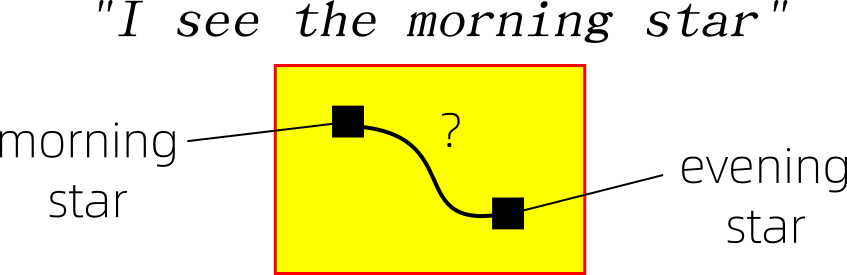
\includegraphics[scale=0.8]{morning-star.png}}}
\end{equation}

又例如 同一个群 可以有不同的 群展示 (group presentations),似乎也可以用 HoTT 处理。

这些 不是 path-connected 的空间 具有 groupoid 结构,可以产生 1-groupoid,2-groupoid 等不同的层级,直至 ∞-groupoid. 这方面我暂时不太理解。

大家可以看到,HoTT 涉及的是「真」的 内部(即黄色方格),但 AGI 主要涉及的是 逻辑的应用,是在 命题空间的 外部(即整个黄色香蕉那空间、其子集空间

之间的映射)。 这并不是说 HoTT 对 AGI 没用,但它的影响是比较 微妙 (subtle) 的,我暂时不能判断。

其实 Transformer 有能力学习非常复杂的 syntactic manipulations,也就是说,它可以隐式地学习各种我们研究的逻辑,例如 modal logic,的推导方式。 如果这样,它似乎可以「绕过」而不需要我们直接 implement 那些麻烦的逻辑形式。 但也有可能是,我们人工地 附加某些 逻辑结构 的 约束,可以加速 深度学习。 这些需要实验证实,是现时非常重要的方向。

\end{minipage}
\end{preview}

\begin{preview}
\begin{textblock*}{5cm}(2.1cm,2.3cm) % {block width} (coords) 
	{\color{red}{\large \textcircled{\small \themypage}}}
	\addtocounter{mypage}{1}
\end{textblock*}

\begin{minipage}{\textwidth}
	\setlength{\parskip}{0.4\baselineskip}

\section{Modal logic and sheaf semantics}

模态逻辑 (modal logic) 与 可能世界语义 (possible world semantics) 是一种很 powerful 的逻辑形式,它可以处理很多哲学逻辑上的课题。 以前我学习符号逻辑 AI 时,比较忽略它,因为要在 计算机上实现 模态逻辑引擎 比较麻烦。  随着 AGI 越来越接近,我觉得有必要更仔细研究一下。

这篇文章的重点是:模态逻辑 具有 层 (sheaf) 和 topos 的结构。 事实上,topos semantics 是逻辑语义学的 「最新」 发展 (其实也很旧了 哈),有说 topos 语义能处理几乎所有我们知道的逻辑语义(究竟有什么例外我也不知)。

以下这个图就是精要: 
\begin{equation}
\vcenter{\hbox{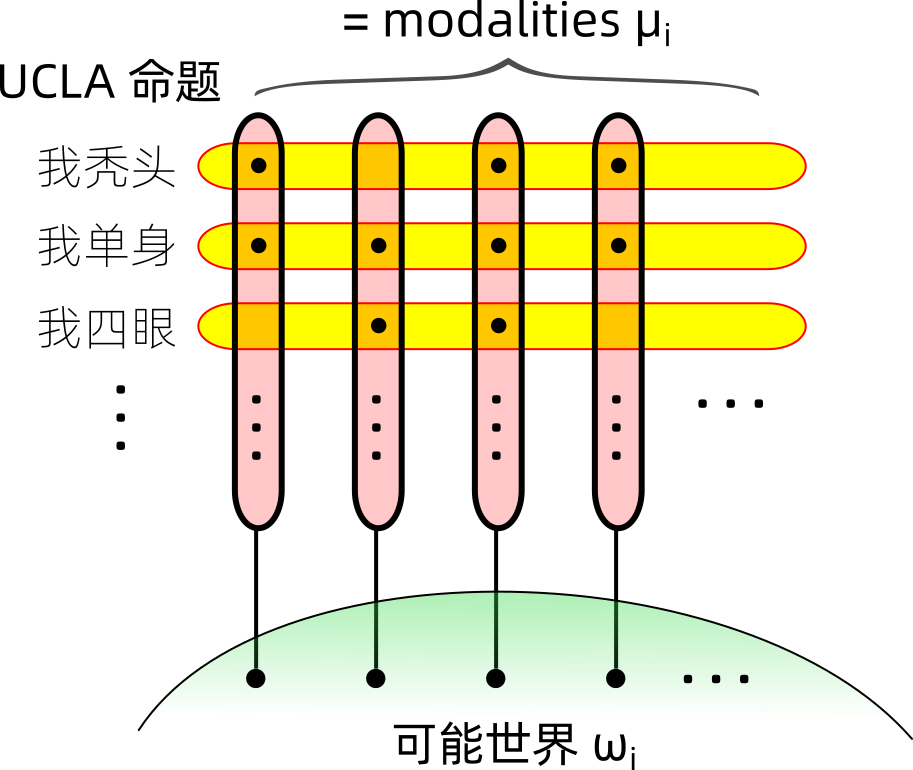
\includegraphics[scale=0.7]{possible-worlds-as-sheaf.png}}}
\end{equation}

\begin{itemize}
	\item 底下的绿色集合 纯粹是 每个可能世界的指标 (index), 例如 N = \{1,2,3,4 \}
	\item 每个蓝色的「冰条」代表一个 可能世界。 它们构成一个 纤维结构 (fibration) 或 层。
	\item 红色横线 表示 每个逻辑命题 在不同的可能世界内的取值情况
	\item Modality = 可能世界 的同义词,在 John L Bell 的书里用这术语
\end{itemize}

但我觉得最精简的论述是这篇 2008 的论文: Topology and Modality: The Topological Interpretation of First-Order Modal Logic by Awodey \& Kishida.  本文主要是基于这篇。

那篇论文的重点是: modal propositional logic 有某种简单的 拓扑语义,而 first-order predicate logic 有另一种 denotational 语义,将两者「乘积」起来,构成 first-order modal logic 的 sheaf 语义。(学过 编程语言语义学 的人可能已听过 denotational semantics.) 我们先分别介绍这两种语义:

\subsection{模态逻辑的拓扑语义}

这是 Tarski-McKinsey 1944年 最先提出的。 想法就是:

\begin{itemize}
	\item 一个 可能世界 对应于 拓扑空间的一个 开集 (open set)
	\item 一个 命题 等同于 其所在为真的可能世界的 集合 (= set of open sets) \\
		这种命题称为「UCLA 命题」,由加州大学的研究者们提出
	\item 模态算符 ⋄ 和 ◻ 分别对应于拓扑上的 closure 和 interior operation
\end{itemize}

举例来说,只考虑下面 4个可能世界,那么「我破脚」并不是必然的,但「我单身」是必然的。「◻ 我单身」这命题的 interior = 全域,所以命题为 真。

\begin{equation}
\vcenter{\hbox{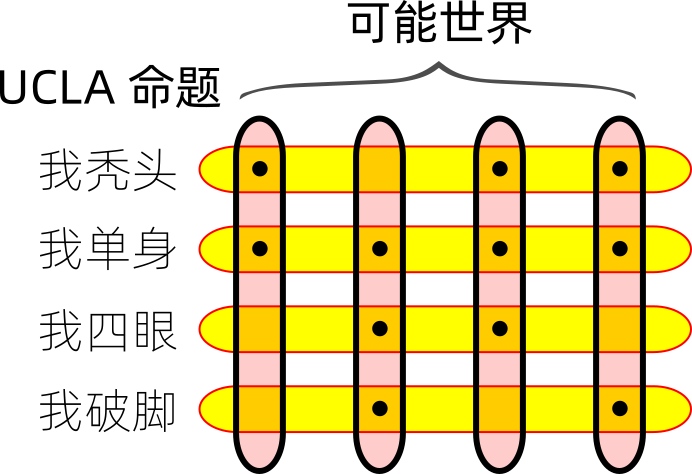
\includegraphics[scale=0.7]{possible-worlds-example.png}}}
\end{equation}

\subsection{谓词逻辑的 denotational 语义}

这部分是比较经典的 模型论 (model theory),我不想花太多时间解释,基本上它用一个 结构  来 诠释 (interpret) 逻辑命题。D 是一个逻辑物体的 论域 (domain),例如 { 苹果,香蕉,橙,John,Mary } 等。 R 是一些 关系 (relations) 或 谓词 (predicates),例如「x 是男人」、「x 喜欢吃 y」等。 f 是一些 函数 (functions),例如「x 的妈妈」、「x 最喜欢的水果 」、等。 c 是一些 常数,例如「c1 = John」等。 一个结构 M 包含足够的资料去 赋值 (interpret) 任何命题的真假。 也可以把 M 看成一个 可能世界 的资料,只是它是唯一的世界而已。
\begin{equation}
\vcenter{\hbox{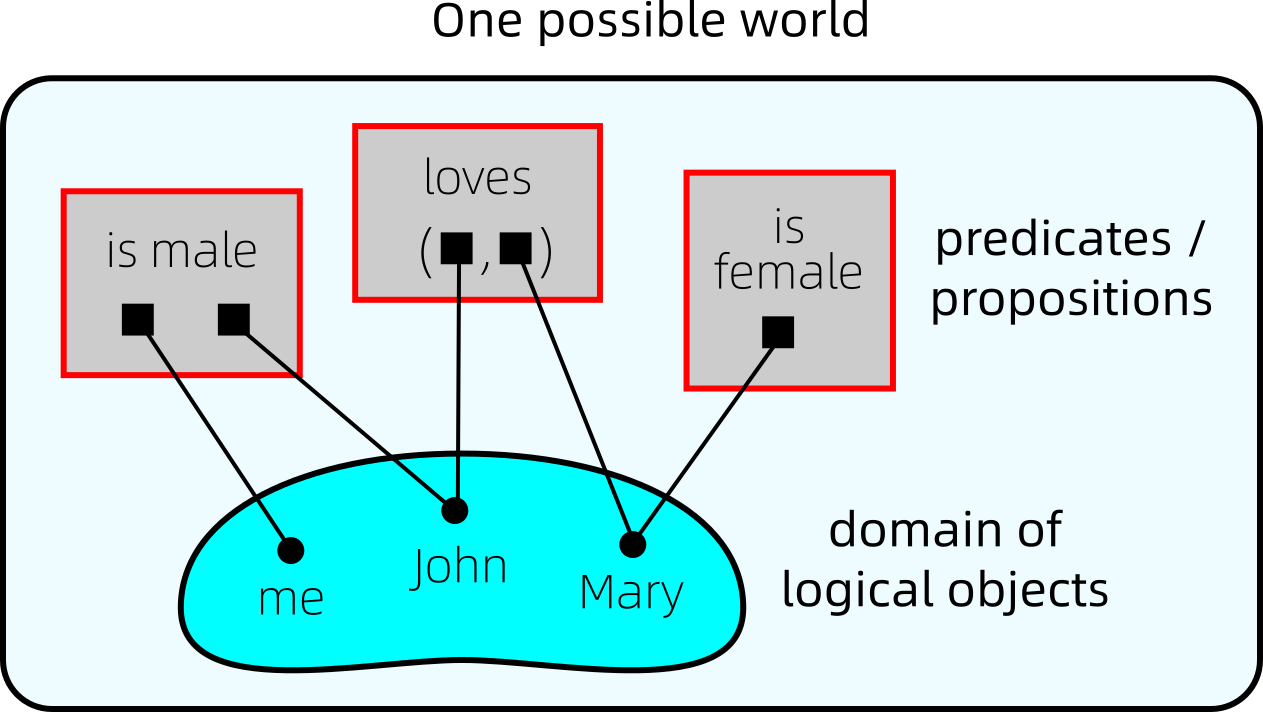
\includegraphics[scale=0.7]{possible-world-single-example.png}}}
\end{equation}

\end{minipage}
\end{preview}

\begin{preview}
\begin{textblock*}{5cm}(2.1cm,2.3cm) % {block width} (coords) 
{\color{red}{\large \textcircled{\small \themypage}}}
\addtocounter{mypage}{1}
\end{textblock*}

\begin{minipage}{\textwidth}
\setlength{\parskip}{0.4\baselineskip}

\subsection{结合 modal 与 first-order 语义}

所谓结合,似乎是一种乘积,或者更简单地就是 将纤维顺着方向并排起来,这是一个 加法:

构成一个 sheaf,而 sheaf 也可以看成是 topos.  整体的图像大概是这样的:
\begin{equation}
\vcenter{\hbox{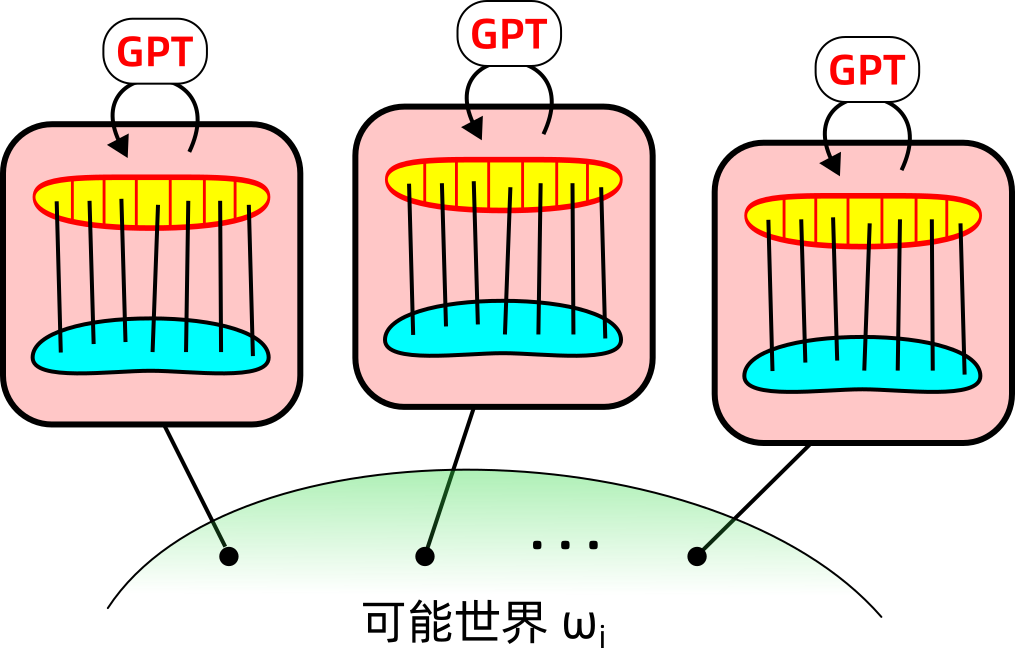
\includegraphics[scale=0.7]{possible-worlds-as-sheaf-with-GPT.png}}}
\end{equation}

\begin{itemize}
	\item 从 人脑 的角度看,它处理「可能世界」的能力是很有限的。 
	\item 最经典的例子是 下棋 时,每个预测的棋步就是一个可能世界。 在一般情况下,人们通常只能预测 3-5 步。
	\item 每个 可能世界 其实跟当前的世界 只相差一个命题,似乎在实践上不必把可能世界想象成「庞然大物」。
	\item 可能世界 是在思考时 动态地 (dynamically) 产生的,我们不可能快速地 根据每个可能世界 训练一个 GPT,因此上面的 GPT's 是同一个训练结果的 拷贝。
	\item 如要实现 模态逻辑 推理,要将上面那个「小 GPT」的功能扩充,让它可以处理多个可能世界的推理。暂时我想到的方法,纯粹是沿用 经典逻辑 AI 的思路,例如将每个可能世界 tag 上特定的命题,然后再计算  
	\item 当可能世界的个数很少时,拓扑 的 closure / interior 概念似乎没有太大的启发性。从 计算机 的角度看,连续空间是很「理想化」的东西,实际上很难实现。

\end{itemize}

这些都算颇直观的,我有空会详细一点看,但现在突然觉得这个方向未必太有用....

\subsection{Some technical details about sheaves}

\end{minipage}
\end{preview}

\begin{preview}
\begin{textblock*}{5cm}(2.1cm,2.3cm) % {block width} (coords) 
	{\color{red}{\large \textcircled{\small \themypage}}}
	\addtocounter{mypage}{1}
\end{textblock*}
	
\begin{minipage}{\textwidth}
	\setlength{\parskip}{0.4\baselineskip}
		
\section{What's the use of all these to AGI?}

		
\end{minipage}
\end{preview}

\end{document}
